\chapter{Preliminaries}
\gls{rl} is intuitively explainable as the process of learning from interaction with the environment, but this hasty explanation is only a very high level description of it; indeed, a more formal way to model the problem is required to properly analyze it. This chapter provides a description of the mathematical framework required to model \gls{rl}. It also explains a selection of algorithms that are related to the work done in this thesis in order to provide enough knowledge about the literature I dealt with during my years of Ph.D. research.

\section{Agent and environment}
\begin{figure}[b]
\begin{minipage}{\textwidth}
\begin{center}
  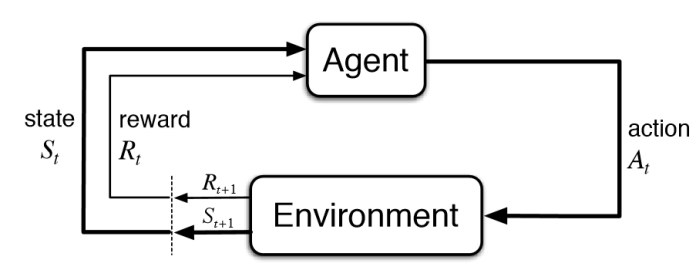
\includegraphics[scale=.75]{img/mdp1.jpg}
\end{center}
\end{minipage}
\caption[Reinforcement Learning problem scheme]{The scheme of a \gls{rl} model.}\label{F:mdp1}
\end{figure}
The interaction of an agent inside an environment can be seen as the execution of actions to move itself in the environment and observing the consequences of its actions (Figure \ref{F:mdp1}). The temporal progress of the interaction is modeled in a set of discrete time steps $t_i$ where the agent sees a representation $s_i$ of the environment, executes an action $a_i$ and observes the new representation of the environment $s_{i+1}$. The problems about observation and interaction discussed in Chapter~\ref{C:intro} are simplified by an explicit selection of data to observe from the environment and of the executable actions. In this way, only the relevant aspect of the sensory data acquired from the environment the agent are used. Together with $s_{i+1}$, the agent also sees a return $r_i$ which is not given by the environment, but it is a measure considered by the agent to evaluate the convenience of the consequences of the actions it executes. The total number of time steps is called \textit{horizon} $H$ and determines a first taxonomy of problems:
\begin{itemize}
 \item finite time horizon: $t_i, \forall i \in [0, 1, 2, \dots, H)$;
 \item infinite time horizon: $t_i, \forall i \in [0, 1, 2, \dots, \infty)$.
\end{itemize}
Some problems can terminate before reaching the horizon, which happens when the agent reaches special situations called \textit{absorbing} states. These states are usually desirable or catastrophic states when the interaction of the agent with the environment is no more useful or impossible. The set of steps between the start of the interaction to the end is called \textit{episode}.

The interaction of the agent with the environment is performed with the purpose to reach a goal for which the agent has been designed. The way to give the knowledge of the goal to the agent is to provide it with a measure of the quality of its behavior. This measure is called \textit{reward} and is a function usually returning a real scalar value given the observation of the current state of the agent. The goal of the agent is to maximize a measure related to the collected rewards. In an infinite time horizon problem it can be:
\begin{itemize}
 \item cumulative reward:
 \begin{equation}\label{E:sumrew}
  J = \sum_{t=0}^\infty r_t;
 \end{equation}
\item average reward:
\begin{equation}
 J = \lim_{n\to\infty}\dfrac{\sum_{t=0}^n r_t}{n};
\end{equation}
\item discounted cumulative reward:
\begin{equation}\label{E:discumrew}
 J = \sum_{t=0}^\infty \gamma^t r_t.
\end{equation}
\end{itemize}
The measure in Equation~\ref{E:discumrew} uses a real scalar $\gamma \in (0, 1]$, called \textit{discount factor}, which has the purpose to give different importance to rewards w.r.t. the time step they have been collected. If $\gamma = 1$ the equation reduces to~\ref{E:sumrew}, whereas the smaller it becomes the less the agent cares about rewards far in time.

\section{Markov Decision Processes}
\begin{figure}[t]
\begin{minipage}{\textwidth}
\begin{center}
  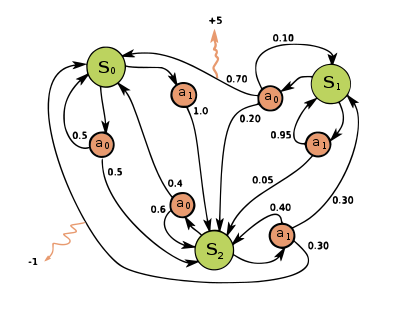
\includegraphics[scale=.6]{img/mdp2.png}
\end{center}
\end{minipage}
\caption[Markov Decision Process]{...}\label{F:mdp2}
\end{figure}
The mathematical framework to study the interaction of the agent with the environment is provided by the theory behind \glspl{mdp}. A \gls{mdp} is defined as a $6$-tuple where $<\mathcal{S}, \mathcal{A}, \mathcal{R}, \mathcal{T}, \gamma, \mu>$:
\begin{itemize}
 \item $\mathcal{S}$ is the set of states where the agent can be in the environment;
 \item $\mathcal{A}$ is the set of actions that the agent can execute in the environment;
 \item $\mathcal{R}$ is the set of rewards obtainable by the agent;
 \item $\mathcal{T}$ is the \textit{transition function} consisting in the probability of reaching a state $s_{t+1}$ executing action $a_t$ in state $s_t$: $\mathcal{T}(s_t, a_t) = P(s_{t+1} | s_t, a_t)$;
 \item $\gamma$ is the discount factor;
 \item $\mu$ is the probability of each state to be the initial one: $\mu(s) = P(s_0 = s)$.
\end{itemize}
A \gls{mdp} is called \textit{finite}, or \textit{discrete}, if the set of states $\mathcal{S}$ and set of actions $\mathcal{A}$ are finite; it is called \textit{infinite}, or \textit{continuous}, when the set of states $\mathcal{S}$ is infinite and/or the set of actions $\mathcal{A}$ is infinite. For facilitating the discussion of the following concepts, let $S_t$, $A_t$ and $R_t$ be respectively the state, executed action and obtained reward of the agent at time step $t$.

\subsection{Value functions}
Recalling that the goal of the agent is to maximize the cumulative (discounted) reward obtained during an episode, a \gls{mdp} is considered \textit{solved} when the agent learns the actions to perform in each state which maximizes this measure. The function defining the probability of executing action $a$ in a state $s$ is called \textit{policy}: $\pi(s) = P(a|s)$. An \textit{optimal} policy $\pi^*$ is the one which, when followed, allows the agent to solve the \gls{mdp}. Considering the stochasticity in the transition function $\mathcal{T}$ and in the policy $\pi$, the expected value of the cumulative discounted reward obtainable following $\pi$ is called \textit{state value function}:
\begin{equation}
 V_\pi(s) = \mathbb{E}_\pi[\sum_{k=0} \gamma^k R_{t+k} | S_t = s], \forall s \in \mathcal{S}.
\end{equation}
Then, an optimal policy can be defined also as the one which maximizes the value function of each state:
\begin{equation}
 V^*(s) = \max_\pi V_\pi(s), \forall s \in \mathcal{S}.
\end{equation}
Together with the state value function, the \textit{action value function} is defined as:
\begin{equation}
 Q_\pi(s, a) = \mathbb{E}_\pi[\sum_{k=0} \gamma^k R_{t+k} | S_t = s, A_t = a], \forall s \in \mathcal{S}, a \in \mathcal{A}.
\end{equation}
And subsequently the optimal policy maximizes also the action value function of each state-action tuple:
\begin{equation}
 Q^*(s,a) = \max_\pi Q_\pi(s,a), \forall s \in \mathcal{S}, a \in \mathcal{A}.
\end{equation}

\subsection{Dynamic Programming}

\subsubsection{Policy Iteration}

\subsubsection{Value Iteration}

\section{Reinforcement Learning to solve MDP}

\subsection{Online}

\subsection{Batch}

\subsection{Deep Reinforcement Learning}
